\documentclass[border=10pt]{standalone}
\usepackage{tikz}
\usetikzlibrary{calc}

\tikzstyle{vertex}=[circle,draw,fill=black!20,minimum size=0.7cm,inner sep=0pt]
\tikzstyle{selected vertex} = [vertex, fill=red!24]
\tikzstyle{edge} = [draw,thick,->]
\tikzstyle{weight} = [font=\small]
\tikzstyle{selected edge} = [draw,->,line width=3pt,blue!70]
\tikzstyle{rev edge} = [draw,->,line width=3pt,red!60]

\begin{document}
\noindent
    \centering
    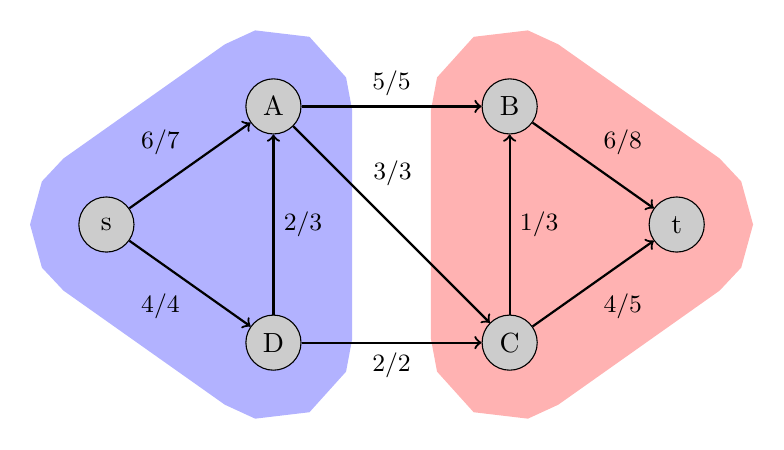
\begin{tikzpicture}[scale=1.0,transform shape,auto,swap]
    \draw[rounded corners, blue!30, line width=2cm] (-2.1213,1.5) -- (0,3) -- (0,0) -- cycle;
    \draw[rounded corners, red!30, line width=2cm] (5.1213,1.5) -- (3,3) -- (3,0) -- cycle;
        \node[vertex] (D) at (0, 0) {D};
        \node[vertex] (C) at (3, 0) {C};
        \node[vertex] (B) at (3, 3) {B};
        \node[vertex] (A) at (0, 3) {A};
        \node[vertex] (s) at (-2.1213, 1.5) {s};
        \node[vertex] (t) at (5.1213, 1.5) {t};
        \path[edge] (D) -- node[weight] {2/2} (C);
        \path[edge] (C) -- node[weight] {1/3} (B);
        \path[edge] (A) -- node[weight,above] {5/5} (B);
        \path[edge] (D) -- node[weight] {2/3} (A);
        \path[edge] (s) -- node[weight,below left] {4/4} (D);
        \path[edge] (s) -- node[weight,above left] {6/7} (A);
        \path[edge] (C) -- node[weight] {4/5} (t);
        \path[edge] (B) -- node[weight,above right] {6/8} (t);
        \path[edge] (A) -- node[weight,above right,pos=0.355] {3/3} (C);
    \end{tikzpicture}
\end{document}
